\chapter{Theory}
\section{Algorithms}
This chapter discusses commonly used algorithms in image processing for edge detection, identifying areas of interest and applying them to pupil detection. At first, the algorithms will be discussed and analyzed on possible use cases, individual strengths and weaknesses. The algorithms use the same preprocessed images from the LPW data, so it is possible to showcase and compare the results. Even though different algorithms are use, the general approach for pupil detection can be summarized by finding the region of interest (ROI), then finding the pupil contour and finally approximating the pupil with an ellipse. Depending on the algorithm, the steps are sometimes extended or even combined. This chapter also discusses the possible combinations of algorithms. 

\subsection{Fundamental notation}\label{subsec:funda}
Throughout this thesis, the following notation are used to describe the algorithms.
The image with intensity level $I$ is a function:

$f(x,y): \mathbb{\mathbb{N_0} }^2 \rightarrow \mathbb{\mathbb{N_0}}$, where $f(x,y)$ is the intensity $I \in $ [$0,255$] at position $(x,y)$

In image processing, the coordinate system is defined differently than in mathematics. The origin is in the upper left corner and the x-axis points vertically down. The y-axis points horizontally to the right. this is shown in figure \ref{fig:coordsystem}.

\begin{figure}[h]
    \centering

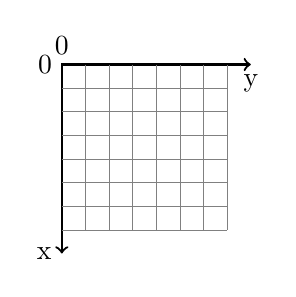
\begin{tikzpicture}[x=0.3cm,y=-0.3cm]
    
    % Draw the x-axis
    \draw[->,thick] (0,8) -- (0,0) -- (8,0) node[below] {y};
    % Draw the y-axis
    \draw[->,thick] (0,0) -- (0,8) node[left] {x};
    % Label the origin
    \node at (0,0) [left] {0};
    \node at (0,0) [above] {0};
    \foreach \x in {1,2,...,7}
    \draw[gray, very thin] (\x,0) -- (\x,7);
  \foreach \y in {1,2,...,7}
    \draw[gray, very thin] (0,\y) -- (7,\y);
  \end{tikzpicture}

    \caption{Coordinate system used in image processing.}
    \label{fig:coordsystem}
\end{figure}

Also important to note is that the image is a discrete function: Therefore, each intensity value $I$ comes with a quantization error. The quantization error is also present when using an algorithm on the image's intensity values or position $(x,y)$. So it is not possible to have an exact result, it is always an approximation of the real result.

\subsubsection{Relationship between pixels}
Another important theory in this thesis will be based on the relationship between pixels. In this subsection, the terms \textbf{neighborhood}, \textbf{adjacency}, \textbf{connectivity}, \textbf{region} and \textbf{boundaries} will be introduced and visualized so that they can be used in the following chapters. 

\paragraph{Neighborhood}
A pixel $P$ at location $(x,y)$ has two vertical neighbor pixels and two horizontal neighbor pixels in a 2D image. These neighbors are defined as $N_4(P)$ with coordinates: 
\begin{equation}
        N_4(P) = \{(x,y+1),(x,y-1),(x+1,y),(x-1,y)\}
\end{equation}
A pixel $P$ at location $(x,y)$ has four diagonal neighbor pixels in a 2D image. These neighbors are defined as $N_D(P)$ with coordinates:
\begin{equation}
    N_D(P) = \{(x+1,y+1),(x+1,y-1),(x-1,y+1),(x-1,y-1)\}
\end{equation}

Combining the neighbors from $N_4(P)$ and $N_D(P)$ results in the 8-neighborhood $N_8(P)$ of pixel $P$:
\begin{equation}
    N_8(P) = N_4(P) \cup N_D(P)
\end{equation}

Those three different types of neighbors are visualized in figure \ref{fig:neighborhoods}.

    \begin{figure}[ht]
        \centering
        \begin{subfigure}[b]{0.23\textwidth}
            \centering
            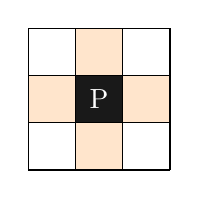
\begin{tikzpicture}[scale=0.6]
                \draw (0,0) grid (3,3);
                \filldraw[fill=orange!20] (1,0) rectangle (2,1);
                \filldraw[fill=orange!20] (1,2) rectangle (2,3);
                \filldraw[fill=orange!20] (0,1) rectangle (1,2);
                \filldraw[fill=orange!20] (2,1) rectangle (3,2);
                \filldraw[fill=black!90] (1,1) rectangle (2,2);
                \node[white] at (1.5,1.5) {P};
            \end{tikzpicture}
            \caption{$N_4(P)$}
            \label{fig:n_4}
        \end{subfigure}%
        \begin{subfigure}[b]{0.23\textwidth}
            \centering
            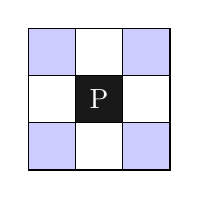
\begin{tikzpicture}[scale=0.6]
                \draw (0,0) grid (3,3);
                \filldraw[fill=blue!20] (0,3) rectangle (1,2);
                \filldraw[fill=blue!20] (2,0) rectangle (3,1);
                \filldraw[fill=blue!20] (0,0) rectangle (1,1);
                \filldraw[fill=blue!20] (2,2) rectangle (3,3);
                \filldraw[fill=black!90] (1,1) rectangle (2,2);
                \node[white] at (1.5,1.5) {P};
            \end{tikzpicture}
            \caption{$N_D(P)$}
            \label{fig:n_d}
        \end{subfigure}%
        \begin{subfigure}[b]{0.23\textwidth}
            \centering
            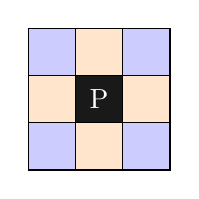
\begin{tikzpicture}[scale=0.6]
                \draw (0,0) grid (3,3);
                \filldraw[fill=blue!20] (0,3) rectangle (1,2);
                \filldraw[fill=blue!20] (2,0) rectangle (3,1);
                \filldraw[fill=blue!20] (0,0) rectangle (1,1);
                \filldraw[fill=blue!20] (2,2) rectangle (3,3);
                \filldraw[fill=orange!20] (1,0) rectangle (2,1);
                \filldraw[fill=orange!20] (1,2) rectangle (2,3);
                \filldraw[fill=orange!20] (0,1) rectangle (1,2);
                \filldraw[fill=orange!20] (2,1) rectangle (3,2);
                \filldraw[fill=black!90] (1,1) rectangle (2,2);

                \node[white] at (1.5,1.5) {P};
            \end{tikzpicture}
            \caption{$N_8(P)$}
            \label{fig:n_8}
        \end{subfigure}%
        \caption{3 different neighborhoods of pixel $P$ at location $(x,y)$.}
        \label{fig:neighborhoods}
    \end{figure}


\paragraph*{Adjacency} There are three types of adjacent pixels in a 2D image. Let $V$ be the set of intensity values used to define adjacency. Depending on the intensity range of the image, it is possible to define different subsets of $V$, containing the intensity values considered adjacent if they are present in the neighborhood. In a binary image, $V$ is often defined as $V$ = $\{1\}$, where $0$ stands for background and $1$ for foreground (This can also be considered a binary mask). In a grayscale image, $V$ can be defined as any subset of the intensity range.

To keep it simple, the following explanations uses a binary image with $V$ = $\{1\}$. Let's define $P$ as a pixel at location $(x,y)$ and $Q$ as a pixel at location $(x',y')$. $P$ and $Q$ are considered adjacent if $Q$ is in the neighborhood of $P$ and $f(Q)$ is $\in V$. These are the three adjacency types:

\begin{itemize}
    \item 4-adjacency, if $Q_i \in N_4(P) and f(Q_i) \in  V$: The pixels directly above, below, left and right of the pixel. 
    \item 8-adjacency, if $Q_i \in N_8(P) and f(Q_i) \in  V$: The pixels directly above, below, left, right and the pixels diagonally adjacent to the pixel.
\end{itemize}
These two adjacency types are visualized in figure \ref{fig:adjacency}.
\begin{equation*}
    \bullet \text{ m-adjacency} \begin{cases}
   \text{if } Q \in N_4(P) \text{ and } f(Q) \in  V \\
    Q \in N_D(P) \text{ and } N_D(P)  \cap N_4(Q) \text{ has no intensities} \in  V
    \end{cases}
    \end{equation*}


    \begin{figure}[ht]
        \centering
        \begin{subfigure}{0.40\textwidth}
            \centering
            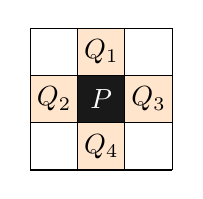
\begin{tikzpicture}[scale=0.6]
                \draw (0,0) grid (3,3);
                \filldraw[fill=orange!20] (1,0) rectangle (2,1);
                \filldraw[fill=orange!20] (1,2) rectangle (2,3);
                \filldraw[fill=orange!20] (0,1) rectangle (1,2);
                \filldraw[fill=orange!20] (2,1) rectangle (3,2);
                \filldraw[fill=black!90] (1,1) rectangle (2,2);


                \node[white] at (1.5,1.5) {$P$};
                \node at (1.5,2.5) {$Q_1$};
                \node at (0.5,1.5) {$Q_2$};
                \node at (2.5,1.5) {$Q_3$};
                \node at (1.5,0.5) {$Q_4$};




            \end{tikzpicture}
            \caption{4-adjacency}
            \label{fig:a_4}
        \end{subfigure}%
        \begin{subfigure}{0.40\textwidth}
            \centering
            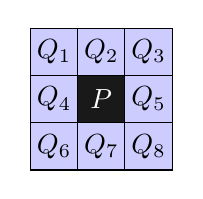
\begin{tikzpicture}[scale=0.6]
                \draw (0,0) grid (3,3);
                \filldraw[fill=blue!20] (0,3) rectangle (1,2);
                \filldraw[fill=blue!20] (2,0) rectangle (3,1);
                \filldraw[fill=blue!20] (0,0) rectangle (1,1);
                \filldraw[fill=blue!20] (2,2) rectangle (3,3);
                \filldraw[fill=blue!20] (1,0) rectangle (2,1);
                \filldraw[fill=blue!20] (1,2) rectangle (2,3);
                \filldraw[fill=blue!20] (0,1) rectangle (1,2);
                \filldraw[fill=blue!20] (2,1) rectangle (3,2);
                \filldraw[fill=black!90] (1,1) rectangle (2,2);
                \node[white] at (1.5,1.5) {$P$};
                \node at (0.5,0.5) {$Q_6$};
                \node at (1.5,0.5) {$Q_7$};
                \node at (2.5,0.5) {$Q_8$};
                \node at (0.5,1.5) {$Q_4$};
                \node at (2.5,1.5) {$Q_5$};
                \node at (0.5,2.5) {$Q_1$};
                \node at (1.5,2.5) {$Q_2$};
                \node at (2.5,2.5) {$Q_3$};
            \end{tikzpicture}
            \caption{$8-adjacency$}
            \label{fig:a_8}
        \end{subfigure}%

        \caption{3 different neighborhoods of pixel $P$ at location $(x,y)$.}
        \label{fig:adjacency}
    \end{figure}
\paragraph{Connectivity}
The connectivity of point $P$ is a set of points that can be reached in $n$ steps with a given adjacency type and intensity set $V$. If point $P$ is connected with $Q$, then there exists a path (or curve) from $P$ to $Q$, that consists of a sequence of distinct pixels with coordinates:
\begin{equation*}
    (x_0,y_0),(x_1,y_1),...,(x_n,y_n), 
\end{equation*}
Where $n$ is the length of the path. If the path is closed then $(x_0,y_0) = (x_n,y_n)$
\paragraph{Region}
Let's define $R$ as a subset of pixels in an image. $R$ is a region if all points $\in R$ are a connected set, meaning that all points in $R$ are connected with each other and therefore form a region. This does not mean that the path connecting all points is closed. Two regions can be adjacent to each other, if their union again forms a connected set. 

\paragraph{Boundary}
The outer boundary of a region $R$ is the set of pixels not in $R$ adjacent to pixels in $R$. In the definition of a boundary, the adjacency type is of importance. As a rule of thumb the 8-adjacency is used to define the boundary. One critical property of the outer boundary is, that it is a closed path. The inner boundary is the set of pixels in $R$ but are 8-adjacent to at least one pixel $\notin  R$. In figure \ref{fig:regbond} it can be seen that the outer boundary is a closed path whereas the inner boundary, in this example identical to the region, is not a closed path.

\begin{figure}[ht]
    \centering
    \begin{subfigure}{0.40\textwidth}
        \centering
        \begin{tikzpicture}
            \matrix [matrix of nodes, nodes in empty cells, nodes={minimum width=1.5em, minimum height=1.5em, draw, thick, anchor=center}, column sep=-\pgflinewidth, row sep=-\pgflinewidth] (M)
            {
                |[fill=gray!20]| & |[fill=gray!20]| & |[fill=gray!20]| & |[fill=gray!20]| & |[fill=gray!20]| & |[fill=gray!20]| & |[fill=gray!20]| \\
                |[fill=gray!20]| & |[fill=gray!20]| & |[fill=gray!20]| & |[fill=red!20]|1 & |[fill=red!20]|1 & |[fill=gray!20]| & |[fill=gray!20]| \\
                |[fill=gray!20]| & |[fill=gray!20]| & |[fill=gray!20]| & |[fill=gray!20]| & |[fill=red!20]|1 & |[fill=red!20]|1 & |[fill=gray!20]| \\
                |[fill=gray!20]| & |[fill=gray!20]| & |[fill=gray!20]| & |[fill=gray!20]| & |[fill=gray!20]| & |[fill=red!20]|1 & |[fill=gray!20]| \\
                |[fill=gray!20]| & |[fill=red!20]|1 & |[fill=gray!20]| & |[fill=gray!20]| & |[fill=red!20]|1 & |[fill=red!20]|1 & |[fill=gray!20]| \\
                |[fill=gray!20]| & |[fill=red!20]|1 & |[fill=red!20]|1 & |[fill=red!20]|1 & |[fill=red!20]|1 & |[fill=gray!20]| & |[fill=gray!20]| \\
                |[fill=gray!20]| & |[fill=gray!20]| & |[fill=gray!20]| & |[fill=gray!20]| & |[fill=gray!20]| & |[fill=gray!20]| & |[fill=gray!20]| \\
            };
            
            \draw [thick] (M-1-1.north west) rectangle (M-7-7.south east);
        \end{tikzpicture}
        
        
            
        \caption{region $R$}
        \label{fig:region}
    \end{subfigure}%
    \begin{subfigure}{0.40\textwidth}
        \centering
        \begin{tikzpicture}
            \matrix [matrix of nodes, nodes in empty cells, nodes={minimum width=1.5em, minimum height=1.5em, draw, thick, anchor=center}, column sep=-\pgflinewidth, row sep=-\pgflinewidth] (M)
            {
                |[fill=gray!20]| & |[fill=gray!20]| & |[fill=red!20]| & |[fill=red!20]| & |[fill=red!20]| & |[fill=red!20]| & |[fill=gray!20]| \\
                |[fill=gray!20]| & |[fill=gray!20]| & |[fill=red!20]| & 1 & 1 & |[fill=red!20]| & |[fill=red!20]| \\
                |[fill=gray!20]| & |[fill=gray!20]| & |[fill=red!20]| & |[fill=red!20]| & 1 & 1 & |[fill=red!20]| \\
                |[fill=red!20]| & |[fill=red!20]|& |[fill=red!20]| & |[fill=red!20]| & |[fill=red!20]| & 1 & |[fill=red!20]| \\
                |[fill=red!20]| & 1 & |[fill=red!20]| & |[fill=red!20]| & 1 & 1 & |[fill=red!20]| \\
                |[fill=red!20]| & 1 & 1 & 1 & 1 & |[fill=red!20]| & |[fill=red!20]| \\
                |[fill=red!20]| & |[fill=red!20]| & |[fill=red!20]| & |[fill=red!20]| & |[fill=red!20]| & |[fill=red!20]| & |[fill=gray!20]| \\
            };
        
            \draw [thick] (M-1-1.north west) rectangle (M-7-7.south east);
        \end{tikzpicture}
        
        \caption{outer boundary (8-adjacent)}
        \label{fig:boundary}
    \end{subfigure}%
    \caption{Region and outer border.}
    \label{fig:regbond}
\end{figure}
\subsection{Preprocessing}
The preprocessing must be defined first to compare the different approaches for pupil detection. The idea behind this step is to create a common ground for narrowing the deviation of the images down so that the algorithms can recreate the same result for different images.

\subsubsection{Converting to grayscale}
As presented in the previous chapter, the iris is the only colorful part of the eye. However, the color itself is of no interest for the detection. Therefore the frames are first converted to grayscale and this is done by converting the images into grayscale. 
In this thesis the grayscale images have the intensity values $I \in [0,255]$ and the image size is depending on the scaling as shown in table \ref{tab:resoluiton}. The scaling is done to reduce the computational cost of the algorithm. 

\begin{table}[h]
    \centering 
    \begin{minipage}{0.7\textwidth}
      \centering
      \begin{tabular}{|c|c|c|}
        \hline
        Scaling &  Shape & numpy array type \\
        \hline
        100\% & 640x480& unit8 \\
        50\% & 320x240 & unit8 \\
        25\% & 160x120 & unit8 \\
        12.5\% & 80x60 & unit8 \\
        6.25\% & 40x30 & unit8 \\
        \hline
      \end{tabular}
      \caption{Scaling of the frames used in this thesis.}
      \label{tab:resoluiton}
    \end{minipage}\hfill
\end{table}

It is important to note that these resolutions are congruent with the LPW paper \cite{zhang_max-planck-institut_nodate}. This is important for the comparison of the results.
When scaling an image, an interpolation is alway done to find the best approximation for the new intensity value $I$ at location $(x,y)$. 

The interpolation used in this thesis is the bilinear interpolation\cite{gonzalez_bilinear_nodate}. This is a linear interpolation in the x and y-axis of the intensity values and solves equation \ref{eq:bilinear}.
\begin{equation}
    v(x,y) = ax + by + cxy + d 
    \label{eq:bilinear}
\end{equation}

Let $Q_{11}=(x_1,y_1)$, $Q_{12}=(x_1,y_2)$, $Q_{21}=(x_2,y_1)$ and $Q_{22}=(x_2,y_2)$ be the four surrounding points. The intensity value $v$ at $(x,y)$ is calculated by equation \ref{eq:bilinear}.The point P at $(x,y)$ is the point of interest. The visualization of the bilinear interpolation is shown in figure \ref{fig:blinearInterpolation}.
\begin{figure}[h]
    \centering
    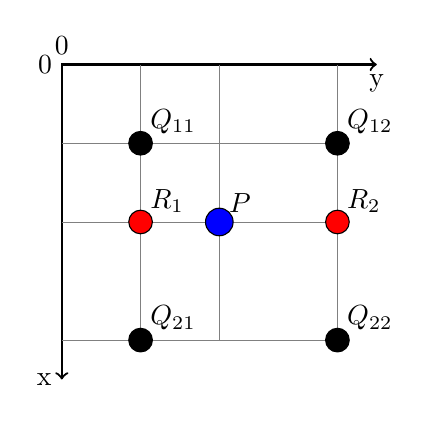
\begin{tikzpicture}[x=0.5cm,y=-0.5cm]
    
    % Draw the x-axis
    \draw[->,thick] (0,8) -- (0,0) -- (8,0) node[below] {y};
    % Draw the y-axis
    \draw[->,thick] (0,0) -- (0,8) node[left] {x};
    % Label the origin
    \node at (0,0) [left] {0};
    \node at (0,0) [above] {0};
    \foreach \x in {2,4,7}
    \draw[gray, very thin] (\x,0) -- (\x,7);
  \foreach \y in {2,4,7}
    \draw[gray, very thin] (0,\y) -- (7,\y);

    \foreach \Point/\PointLabel in {(7,4)/R_2,(2,4)/R_1}
    \draw[fill=red] \Point circle (0.3) node[above right] {$\PointLabel$};

    \foreach \Point/\PointLabel in {(2,2)/Q_{11}, (7,2)/Q_{12}, (2,7)/Q_{21}, (7,7)/Q_{22}}
    \draw[fill=black] \Point circle (0.3) node[above right] {$\PointLabel$};

    \foreach \Point/\PointLabel in {(4,4)/P }
    \draw[fill=blue] \Point circle (0.35) node[above right] {$\PointLabel$};

  \end{tikzpicture}

    \caption{Bilinear interpolation.}
    \label{fig:blinearInterpolation}
\end{figure}

First the intensity values $I_1 = f(R_1)$ and $I_2 = f(R_2)$ are calculated. $f(R_1)$ is the linear interpolation between $Q_{11}$ and $Q_{21}$
\begin{equation}
    f(R_{1}) \approx \frac{x_{2}-x}{x_{2}-x_{1}}f(Q_{11})+\frac{x-x_{1}}{x_{2}-x_{1}}f(Q_{21}) = R_{1}(x,y_{1})
\end{equation}
 $f(R_2)$ is the linear interpolation between $Q_{12}$ and $Q_{22}$.
 \begin{equation}
    f(R_{2}) \approx \frac{x_{2}-x}{x_{2}-x_{1}}f(Q_{12})+\frac{x-x_{1}}{x_{2}-x_{1}}f(Q_{22}) = R_{2}(x,y_{2})
\end{equation}
 Then the intensity value $I = f(P)$ at $P$ is calculated by the linear interpolation between $R_1$ and $R_2$. 
\begin{equation}
    f(P) \approx \frac{y_{2}-y}{y_{2}-y_{1}}f(R_{1})+ \frac{y-y_{1}}{y_{2}-y_{1}}f(R_{2}) = v(x,y)
\end{equation}
Therefore $f(P) = v(x,y)$ is the intensity value at $P$ calculated with the bilinear interpolation of $Q_{11}$, $Q_{12}$, $Q_{21}$ and $Q_{22}$ at $P$.



\subsubsection{Histogram equalization }
Another vital aspect of preprocessing the frames is using Histogram equalization \cite{noauthor_opencv_nodate}. Histogram equalization has the effect of increasing the contrast of the image. This thesis uses Contras Limited Adaptive Histogram Equalization (CLAHE). CLAHE is a histogram equalization method that has the benefit that it is adaptive to the local contrast of the image. Local contrast equalization is very useful if the contrast of the image is not uniform in all regions of the image. Using Histogram Equalization adds additional noise to the image. The additional noise can be dealt with using a low pass filter, like a Gaussian filter for example, to minimize the noise. 

 Using a standard Histogram Equalization approach would lead to a loss of information in the region around the pupil and the iris because this is the region with the highest contrast already. Therefore, more noise would be added to the pupil and iris region. The CLAHE method splits the image into smaller blocks called "tiles". CLAHE then calculates the histogram equalization on each block individually without losing the same amount of information in the pupil region compared to the standard histogram equalization. The CLAHE method is applied to the frames after they are converted to grayscale. The result of this step is shown in figure \ref{fig:clahe}. 

\begin{figure}[h]
    \centering
    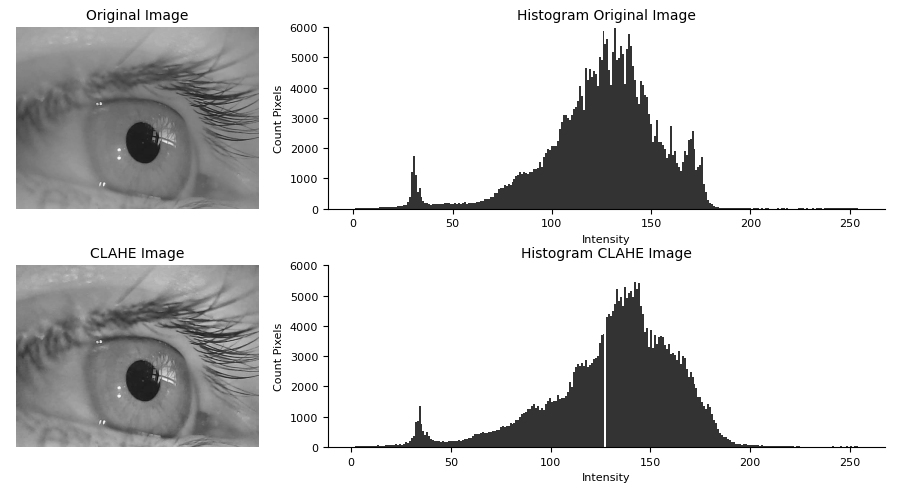
\includegraphics[width=1\textwidth]{plots/clahe.png}
    \caption{Example of CLAHE an its effect on the histogram.}
    \label{fig:clahe}
\end{figure}

\subsection{Edge Detection}
The main goal behind edge detection is to find edges in the image. An edge is defined as a region with high contrast to its surrounding pixels, in other words, a rapid change of intensity in a small area. Edge detection is helpful to filter the image for possible pupil contours. The edge detection analysis is based on a gradient calculation. There are different methods to calculate the gradient of an image. One of the most popular methods is the Sobel operator, which uses the first differential of the intensity change in the image. The Laplacian operator is another method that uses the second differential of the intensity change in the image. In this thesis the Sobel operator is used to calculate the gradient of the image. 
After calculating the gradient, Canny edge detection is used to refine the edges. Canny edge detection is a multi-step algorithm that uses hysteresis thresholding to filter the edges. The edge detection result is a one pixel thick binary edge map.  These edges are now possible candidates for the pupil contour and need additional processing steps to find the pupil contour. 
\subsubsection{Sobel Operators}
The Sobel Operators \cite{gonzalez_sharpening_nodate} is commonly used for edge detection. It is a gradient calculation that uses two 3x3 differential kernels to calculate the gradient of the image. The Sobel gradient is calculated in the x and y direction with their corresponding kernels $k_x$ and $k_y$, and the kernels are defined as:
\begin{center}
    \begin{minipage}{0.44\textwidth}
        \begin{equation}
            k_x = \begin{bmatrix}
                -1 & 0 & +1 \\
                -2 & 0 & +2 \\
                -1 & 0 & +1
            \end{bmatrix} 
        \end{equation}
    \end{minipage}
    \hfill
    \begin{minipage}{0.44\textwidth}
        \begin{equation}
            k_y = \begin{bmatrix}
                -1 & -2 & -1 \\
                0 & 0 & 0 \\
                +1 & +2 & +1
            \end{bmatrix} 
        \end{equation}
         
    \end{minipage}
    
\end{center}
     The gradient vector is $\nabla f(x,y) = [G_x, G_y]^T$  and is calculated by convolving the image $f(x,y)$ with the Sobel kernels $k_x$ and $k_y$.
     \begin{align}
        G_x(x,y) & = f(x,y) * k_x  = \sum_{s=-a}^{a} \sum_{t=-b}^{b} k_x(s,t) f(x+s,y+t) \\
        G_y(x,y) & = f(x,y) * k_y  = \sum_{s=-a}^{a} \sum_{t=-b}^{b} k_y(s,t) f(x+s,y+t)
    \end{align}
     
    $G_x(x,y) = \partial f/ \partial x$ and $G_y(x,y)= \partial f/ \partial y$ are the gradients in x and y direction and the total gradient magnitude $G$ of the gradient vector is calculated with the euclidean norm: 
    \begin{equation}
        G = \sqrt{G_x^2 + G_y^2}
        \label{eq:gradientmagnitude}
    \end{equation} 
    the orientation $\theta$ of the gradient is :
    \begin{equation}
        \theta = \arctan2{\frac{G_y}{G_x}}
        \label{eq:gradientdirection}
    \end{equation}
    The result of the gradient calculation can be seen here:
    \begin{figure}[ht]
        \centering
        % First row: 3 images
        \begin{subfigure}{.33\textwidth}
          \centering
          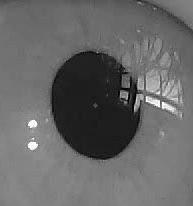
\includegraphics[width=.9\linewidth]{plots/eye_dataset/roi.png}
          \caption{Image of ROI}
          \label{fig:roig}
        \end{subfigure}%
        \begin{subfigure}{.33\textwidth}
          \centering
          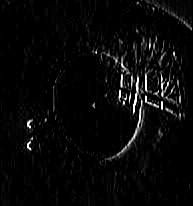
\includegraphics[width=.9\linewidth]{plots/eye_dataset/sx.png}
          \caption{Gradient in x\textbf{$G_{x}$}}
          \label{fig:sx}
        \end{subfigure}%
        \begin{subfigure}{.33\textwidth}
          \centering
          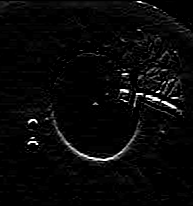
\includegraphics[width=.9\linewidth]{plots/eye_dataset/sy.png}
          \caption{Gradient in y \textbf{$G_{y}$}}
          \label{fig:sy}
        \end{subfigure}
        % Second row: 2 images
        \begin{subfigure}{.33\textwidth}
          \centering
          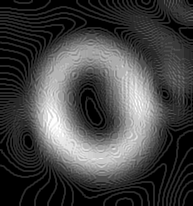
\includegraphics[width=.9\linewidth]{plots/eye_dataset/mag.png}
          \caption{Magnitude \textbf{$G$}}
          \label{fig:mag}
        \end{subfigure}%
        \begin{subfigure}{.33\textwidth}
          \centering
          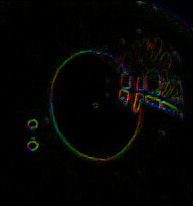
\includegraphics[width=.9\linewidth]{plots/eye_dataset/direction.png}
          \caption{Orientation \textbf{$\theta$}}
          \label{fig:orientation}
        \end{subfigure}
        \caption{Plot of gradient characteristics of the ROI.}
        \label{fig:gradient}
        \end{figure}
    Important to note is that figure \ref{fig:mag} and figure \ref{fig:orientation} are the results of a strong gaussian blurred initial image. 
    \subsubsection{Canny Edge Detection } 
    The Canny Edge Detection \cite{gonzalez_canny_nodate}calculates a single edge points from the gradient vector image.  
    Canny edge detection can summarized in four steps: 
    \begin{enumerate}
        \item Noise reduction, smoothing the image with a Gaussian filter
        \item Compute the gradient magnitude and direction
        \item Non-maximum suppression to the gradient magnitude image
        \item Use double thresholding and connectivity analysis to detect and link edges
    \end{enumerate}
\textbf{Step 1: Noise reduction} \\
The first step is to reduce noise from the input image. This is done by convolving the image with a low pass filter. For this task a Gaussian filter is used. The Gaussian filter is:
\begin{equation}
    f_{filter}(x,y) = \frac{1}{2\pi\sigma^2}e^{-\frac{x^2+y^2}{2\sigma^2}}
\end{equation}
The Gaussian filter is then convolved with the image to smooth the image. 
\begin{equation}
    f_{smoothed}(x,y) = f(x,y) * f_{filter}(x,y)
\end{equation} 

\textbf{Step 2: Compute the gradient magnitude and direction} \\
The gradient magnitude $G$ is calculated with equation \ref{eq:gradientmagnitude} and the gradient direction $\theta$ is calculated with equation \ref{eq:gradientdirection}.

\textbf{Step 3: Non-maximum suppression} \\
The non-maximum suppression is used to thin the edges out so the edges are only one pixel wide. This can be achieved with a loop iterating over all edge pixels and individually checking if the current pixel is the local maximum in the gradient vector's direction $\pm \theta$. If the pixel indeed is the local maximum, the pixel is kept, otherwise it is set to zero. Because as already described in \ref{subsec:funda} the coordinate system is defined different. The gradient direction $\theta$ is in reference to the $x$ axis

\begin{figure}[h]
    \centering
        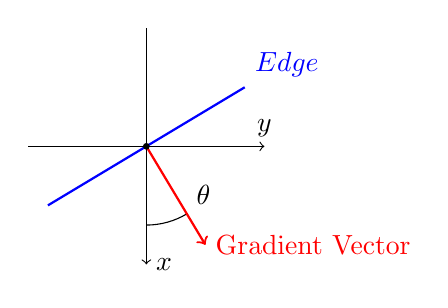
\begin{tikzpicture}[rotate=-90, scale= 0.5]
            % Draw the coordinate axes
            \draw[->] (-3,0) -- (3,0) node[right] {$x$};
            \draw[->] (0,-3) -- (0,3) node[above] {$y$};
            % Draw the first line
            \draw (2,0) arc (0:31:2)node[above right] {$\theta$};
            \draw[->,red,thick] (0,0) -- (2.5,1.5)node[right] {Gradient Vector};
            % Draw the angle marker
        
        ;
            % Draw the second line
            \draw[blue,thick] (1.5,-2.5) -- (-1.5,2.5)node[above right] {$Edge$};
            % Draw the origin
            \filldraw[black] (0,0) circle (2pt);
        \end{tikzpicture}
        \caption{Definition of the gradient direction}
        \label{fig:Definition_grad}
\end{figure}
Because an image is quantized, this also means that $\theta$ needs to be quantized in four directions to evaluate their neighbors. 

\begin{figure}[h]
    \centering
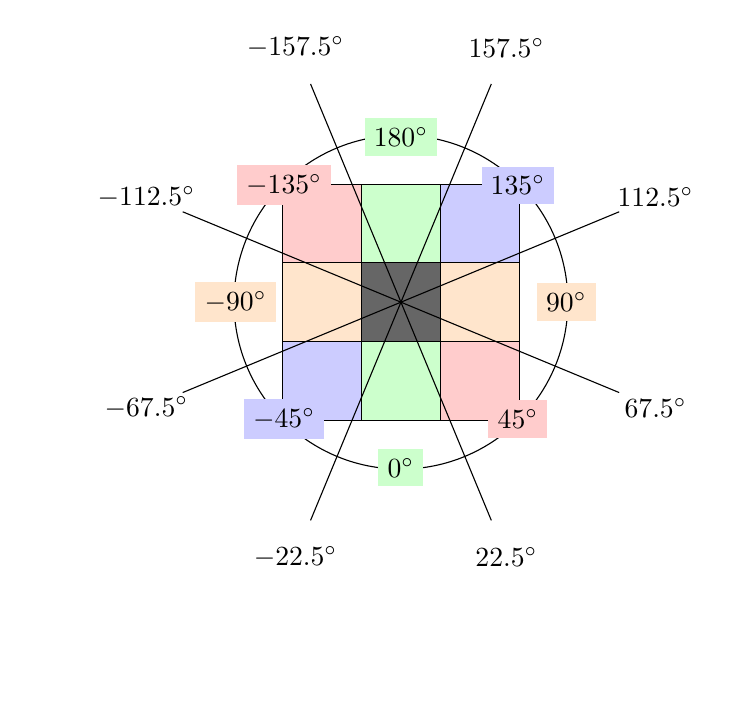
\begin{tikzpicture}[x=1cm,y=1cm]
    % Draw the grid
    \draw (0,0) grid (3,3);
     % Draw unit circle around grid

    % Fill the center pixel with light gray
    \filldraw[fill=blue!20] (0,0) rectangle (1,1);
    \filldraw[fill=blue!20] (2,2) rectangle (3,3);
    \filldraw[fill=orange!20] (0,1) rectangle (1,2);
    \filldraw[fill=orange!20] (2,1) rectangle (3,2);
    \filldraw[fill=red!20] (0,3) rectangle (1,2);
    \filldraw[fill=red!20] (2,0) rectangle (3,1);
    \filldraw[fill=green!20] (1,0) rectangle (2,1);
    \filldraw[fill=green!20] (1,2) rectangle (2,3);
    \filldraw[fill=black!60] (1,1) rectangle (2,2);


    \draw (1.5, 1.5) circle [radius=2.12];
    % Mark angles in 45° steps
    \foreach \ang in {157.5,112.5,67.5,22.5,-22.5,-67.5,-112.5,-157.5} {
        \draw (\ang-90:3.5) ++(1.5,1.5) node [fill=white] {$\ang^\circ$};
        \draw (\ang-90:3) ++(1.5,1.5) -- (1.5,1.5) ;

    }
    \foreach \ang in {0,180} {
        %\draw[thick,green] (\ang-90:2.3) ++(1.5,1.5) -- (1.5,1.5) ;
        \draw (\ang-90:2.1) ++(1.5,1.5) node [fill=green!20] {$\ang^\circ$};

    }

    \foreach \ang in {-45,135} {
        %\draw[thick,blue] (\ang-90:2.3) ++(1.5,1.5) -- (1.5,1.5) ;
        \draw (\ang-90:2.1) ++(1.5,1.5) node [fill=blue!20] {$\ang^\circ$};


    }
    \foreach \ang in {-90,90} {
        %\draw[thick,orange] (\ang-90:2.3) ++(1.5,1.5) -- (1.5,1.5) ;
        \draw (\ang-90:2.1) ++(1.5,1.5) node [fill=orange!20] {$\ang^\circ$};


    }
    \foreach \ang in {45,-135} {
        %\draw[thick,red] (\ang-90:2.3) ++(1.5,1.5) -- (1.5,1.5) ;
        \draw (\ang-90:2.1) ++(1.5,1.5) node [fill=red!20] {$\ang^\circ$};


    }

         % Add a tick at 45 degrees

\end{tikzpicture}
  \caption{Quantization of the gradient direction}
  \label{fig:non_max}
\end{figure}
This leads to following quantizations: 
\begin{equation}
    \theta_q = \begin{cases}
    90, & \text{if } 67.5^\circ < \theta \leq 112.5^\circ \, \vee \, -112.5^\circ < \theta \leq -67.5^\circ \\
    -45^\circ, &\text{if }22.5^\circ < \theta \leq 67.5^\circ \, \vee \, -157.5^\circ < \theta \leq -112.5^\circ \\
    +45^\circ, &\text{if }112.5^\circ <\theta \leq 157.5^\circ \, \vee \, -67.5^\circ < \theta \leq -22.5^\circ \\
    0^\circ, &\text{if }-22.5^\circ <\theta \leq 22.5^\circ \, \vee \, -157.5^\circ < \theta \leq 157.5^\circ \\
\end{cases} 
\label{eq:quantization_d}
\end{equation}
It is important to note that two neighboring pixels are used to evaluate the gradient magnitude maximum. This is shown in figure \ref{fig:non_max} and \ref{fig:neighbors}.
Suppose the maximum gradient magnitude is at the current pixel at $(x,y)$, meaning it is a local maximum in the previously defined neighborhood with respect to the gradient direction, the value of the pixel is written into $g_n(x,y)$. Otherwise, it is set to zero $g_n(x,y) = 0$. $g_n(x,y)$ is the non-maximum suppressed edge image. Therefore $g_n(x,y)$ contains only the thinned edges.  

\begin{figure}[ht]
    \centering
    \begin{subfigure}[b]{0.23\textwidth}
        \centering
        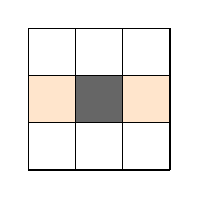
\begin{tikzpicture}[scale=0.6]
            \draw (0,0) grid (3,3);
            \filldraw[fill=orange!20] (0,1) rectangle (1,2);
            \filldraw[fill=orange!20] (2,1) rectangle (3,2);
            \filldraw[fill=black!60] (1,1) rectangle (2,2);
        \end{tikzpicture}
        \caption{Neighbors: 90°}
        \label{fig:n90}
    \end{subfigure}%
    \begin{subfigure}[b]{0.23\textwidth}
        \centering
        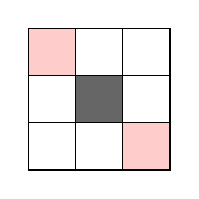
\begin{tikzpicture}[scale=0.6]
            \draw (0,0) grid (3,3);
            \filldraw[fill=red!20] (0,3) rectangle (1,2);
            \filldraw[fill=red!20] (2,0) rectangle (3,1);
            \filldraw[fill=black!60] (1,1) rectangle (2,2);
        \end{tikzpicture}
        \caption{Neighbors: 45°}
        \label{fig:n45}
    \end{subfigure}%
    \begin{subfigure}[b]{0.23\textwidth}
        \centering
        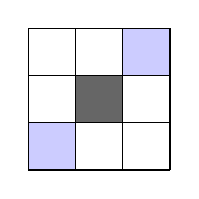
\begin{tikzpicture}[scale=0.6]
            \draw (0,0) grid (3,3);
            \filldraw[fill=blue!20] (0,0) rectangle (1,1);
            \filldraw[fill=blue!20] (2,2) rectangle (3,3);
            \filldraw[fill=black!60] (1,1) rectangle (2,2);
        \end{tikzpicture}
        \caption{Neighbors: -45°}
        \label{fig:nn45}
    \end{subfigure}%
    \begin{subfigure}[b]{0.23\textwidth}
        \centering
        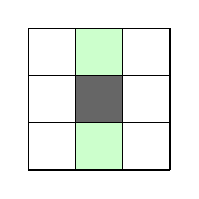
\begin{tikzpicture}[scale=0.6]
            \draw (0,0) grid (3,3);
            \filldraw[fill=green!20] (1,0) rectangle (2,1);
            \filldraw[fill=green!20] (1,2) rectangle (2,3);
            \filldraw[fill=black!60] (1,1) rectangle (2,2);
        \end{tikzpicture}
        \caption{Neighbors: 0°}
        \label{fig:n0}
    \end{subfigure}
    \caption{The gradient magnitude is evaluated in the direction of the gradient.}
    \label{fig:neighbors}
\end{figure}

  

\textbf{Step 4: Double thresholding and connectivity analysis} \\
After Step 3, $g_n(x,y)$ still contains edges that can be thicker than one pixel. $g_n(x,y)$ is then thresholded with a high a low threshold value (hysteresis thresholding), creating two images: 
\begin{equation}
    g_{low}(x,y) = \begin{cases}
    g_n(x,y), & \text{if } g_n(x,y) \geq T_{low} \\
    0, &\text{otherwise}
\end{cases}
\end{equation}
\begin{equation}
    g_{high}(x,y) = \begin{cases}
    g_n(x,y), & \text{if } g_n(x,y) \geq T_{high} \\
    0, &\text{otherwise}
\end{cases}
\end{equation}
Because two different thresholds are used, there is still an overlap between $g_{low}$ and $g_{high}$ edges. All non-zero pixels in $g_{high}$ are considered strong edge pixels. To find all weak edge pixels, the strong edge pixels are substracted from $g_{low}$. 
\begin{equation}
    g_{weak}(x,y) = g_{low}(x,y) - g_{high}(x,y)
\end{equation}
The remaining pixels are considered weak edge pixels.

The next step is to connect the weak edge pixels to the strong edge pixels. This is done by checking the 8-neighborhood of each strong edge pixel. If there is a weak edge pixel in the neighborhood, it is considered a strong edge pixel. This continues until no more weak edge pixels are found. The result is a binary image $g_{final}(x,y)$ containing connected edges. $g_{final}(x,y)$ still doesn't consists of one-pixel thick edges. 

An edge-thinning algorithm solves this problem and returns the wanted image with only one-pixel thick edges. Let's define the edges as set A and a structuring element as B. 
The equation for thinning is: 
\begin{equation}
    A \otimes   B = A - (A \circledast B)
\end{equation}
Where $\otimes$ is the thinning operator, $\circledast$ is the dilation operator.

\paragraph{Results}
In a frame where the pupil region is clearly distinguishable from the rest, the Canny edge detector can be used to find the pupil boundary. But as soon as more noise to the pupil is added, the hysteresis thresholding becomes more tricky and the detection accuracy decreases immensely. Also is it not possible to differentiate between the eye leashes, eyebrows and the pupil. Therefore by using only the Canny edge detector. The pupil edges can not be found reliable and the algorithm itself is not adaptable to a great variety of environments. The problem with Canny edge detection is visualized in figure \ref{fig:canny_clear} and \ref{fig:canny_eyelid}.


\begin{figure}[ht]
    \centering
    \begin{subfigure}{.5\textwidth}
      \centering
      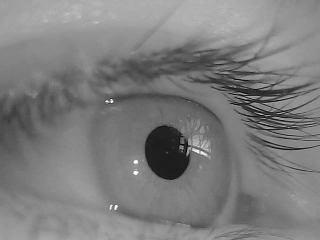
\includegraphics[width=.9\linewidth]{plots/orig_canny.png}
      \caption{Original image, scaling 0.5}
      \label{fig:orig_canny}
    \end{subfigure}%
    \begin{subfigure}{.5\textwidth}
      \centering
      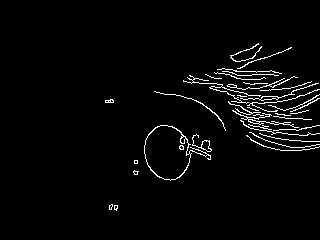
\includegraphics[width=.9\linewidth]{plots/canny.png}
      \caption{Clear pupil region, Canny edge detection}
      \label{fig:canny_region_clear}
    \end{subfigure}
    \caption{Canny edge detection on a clear pupil region}
    \label{fig:canny_clear}
\end{figure}

\begin{figure}[ht]
    \centering
    \begin{subfigure}{.5\textwidth}
      \centering
      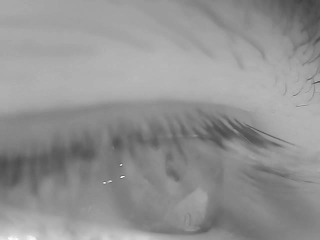
\includegraphics[width=.9\linewidth]{plots/orig_canny_eyelids.png}
      \caption{Original image, scaling 0.5}
      \label{fig:orig_canny_lids}
    \end{subfigure}%
    \begin{subfigure}{.5\textwidth}
      \centering
      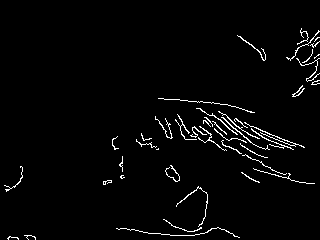
\includegraphics[width=.9\linewidth]{plots/canny_eyelids.png}
      \caption{Weak pupil region, Canny edge detection}
      \label{fig:canny_eyelid}
    \end{subfigure}
    \caption{Canny Edge detection on a frame with weak pupil region}
    \label{fig:canny_eyelid}
\end{figure}

\subsection{Haar like feature detection }
\label{subsec:haar}
\subsubsection{Concept }
Haar-like features \cite{viola_rapid_nodate} is based on the observation that object have a certain local intensity variation in an image and this fact can be useful to identify objects. Haar like features makes use of this and divides the image into rectangular regions and then calculates the difference between the sum of the pixels in the white and gray regions, show in figure \ref{fig:haar_features}. This is done for all possible rectangular positions in the image. The result is a response matrix that is used to classify the image and give insight about the position of the object. In theory the feature is convolved with the image to calculate the response matrix but to make the detection faster, the integral image is calculated once and then used to calculate the response matrix at each possible position in the image.
 This leads to an easy calculation of the response matrix than now only needs four values to be calculated. 
The properties of the different features bring different abilities to detect specific local intensity patterns that are an indicator for a certain object or image region property. 
\subsubsection{Features characteristics}
To get a better understanding of the different features and their characteristics of the resulting response matrix the four features are explained a little more in detail. 
\paragraph{}
\begin{figure}[h]
    \centering
    
    \begin{subfigure}{0.45\textwidth}
        \centering
        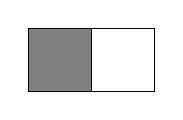
\begin{tikzpicture}[scale=0.8, transform shape]
            % Haar-like feature: Two-rectangle feature
            \draw[fill=gray] (0,0) rectangle (1,1);
            \draw[fill=white] (1,0) rectangle (2,1);
        \end{tikzpicture}
        \caption{Two-Rectangle Feature}
        \label{fig:haar_feature_1}
    \end{subfigure}
    \hfill
    \begin{subfigure}{0.45\textwidth}
        \centering
        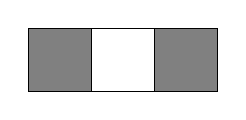
\begin{tikzpicture}[scale=0.8, transform shape]
            % Haar-like feature: Three-rectangle feature
            \draw[fill=gray] (0,0) rectangle (1,1);
            \draw[fill=white] (1,0) rectangle (2,1);
            \draw[fill=gray] (2,0) rectangle (3,1);
        \end{tikzpicture}
        \caption{Three-Rectangle Feature}
        \label{fig:haar_feature_2}
    \end{subfigure}
    
    \vspace{1.5em}
    
    \begin{subfigure}{0.45\textwidth}
        \centering
        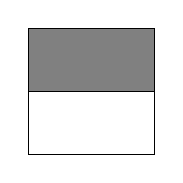
\begin{tikzpicture}[scale=0.8, transform shape]
            % Haar-like feature: Line feature (Horizontal)
            \draw[fill=gray] (0,0) rectangle (2,1);
            \draw[fill=white] (0,-1) rectangle (2,0);
        \end{tikzpicture}
        \caption{Horizontal Line Feature}
        \label{fig:haar_feature_3}
    \end{subfigure}
    \hfill
    \begin{subfigure}{0.45\textwidth}
        \centering
        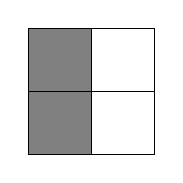
\begin{tikzpicture}[scale=0.8, transform shape]
            % Haar-like feature: Four-rectangle feature
            \draw[fill=gray] (0,0) rectangle (1,1);
            \draw[fill=white] (1,0) rectangle (2,1);
            \draw[fill=gray] (0,1) rectangle (1,2);
            \draw[fill=white] (1,1) rectangle (2,2);
        \end{tikzpicture}
        \caption{Four-Rectangle Feature}
        \label{fig:haar_feature_4}
    \end{subfigure}
    
    \caption{Haar-like Features}
    \label{fig:haar_features}
\end{figure}

The key concept to keep in mind is, that the features generate a response based on the difference of the sum of the pixels in the white and gray regions and therefore are able to detect local intensity patterns. The response of each feature also depends on the size of the feature and stands in relation to the size of the object that is to be detected. The result of the Haar-like features provides information about the presence or absence of a certain pattern that is reflected in the structure of the feature used. Because an object can have more than one fitting feature, the features are often used in a cascade of classifiers. The first classifier is a very simple classifier that is able to detect a lot of features. The following classifiers are more complex and are only used if the previous classifier was able to detect a certain feature. This leads to a very fast detection of the object. This safes computational resources and time. Often Machine learning is involved to classify if an object is present or not, based on the response matrix. 

\subsubsection{Haar-Like Feature for pupil detection }
One very useful feature for finding a point in the pupil is given by a feature described in the paper \cite{swirski_robust_2012} . This feature is constructed differently but is used the same way as the other features to calculate a response matrix. The feature is constructed as following: 
\begin{figure}
    \centering
    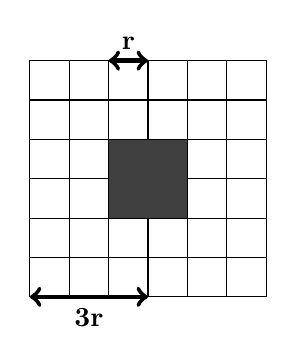
\begin{tikzpicture}[scale=0.5]

        % Grid
        \foreach \x in {0,1,...,5} {
            \foreach \y in {0,1,...,5} {
                \draw (\x,\y) rectangle ++(1,1);
            }
        }
    
        % Center 2x2 area
        \draw[fill=black!75] (2,2) rectangle ++(2,2);
        


       % Measurement on top
    \draw[<->, ultra thick] (0,0) -- (3,0) node[midway, below, font=\bfseries] {3r};

    % Measurement at the bottom
    \draw[<->, ultra thick] (2,6) -- (3,6) node[midway, above, font=\bfseries] {r};
    
    \end{tikzpicture}
\label{haar_pupil}
\caption{Haar-like feature for pupil detection}
\end{figure}
The total size of the feature is $6rx6r$ where the center is of the size $2rx2r$. The feature mimics the shape of an pupil with a larger boundary around it that mimics a lighter iris. The radius is variable and makes it possible to detect the best response to different pupil sizes. The feature is then used to calculate the response matrix and over all different radii and the position with the best response can be considered to be inside the pupil.

\subsection{Thresholding and Ellipse fitting}
\subsubsection{Thresholding}
In Thresholding the characteristic of the pupil is used, that it is the darkest part of the eye as seen in \ref{fig:hist1} . Here it is important to find a certain thresholding value to only extract the pupil. Considering the best scenario that the pupil is not affected by too much noise: no eyelash, no reflection. This method can be reliable to find the pupil region. This process shows to be less computation expensive and finds the pupil fast. 

The most difficult part is to find a fitting threshold value. This could be done by using the histogram of the frame. When inspecting the histogram, one could consider the lowest peak in the histogram as the given center value for thresholding. But this is not always the case. There is also the possibility for adaptive thresholding for example otsu thresholding. but throughout the work with thresholding otsu was also tested but was found to be less reliable than the histogram approach itself. 

\begin{figure}[ht]
    \centering
    \begin{subfigure}{.5\textwidth}
      \centering
      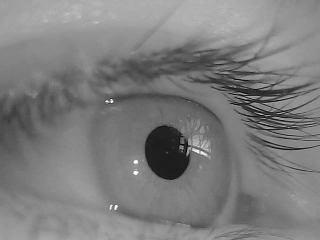
\includegraphics[width=.9\linewidth]{plots/orig_canny.png}
      \caption{Original frame}
      \label{fig:th_orig}
    \end{subfigure}%
    \begin{subfigure}{.5\textwidth}
      \centering
      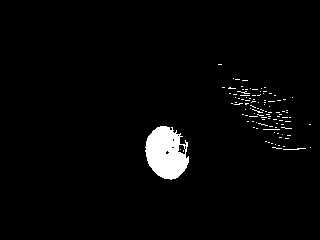
\includegraphics[width=.9\linewidth]{plots/thresholded.jpg}
      \caption{thresholded frame}
      \label{fig:th_thres}
    \end{subfigure}
    \caption{Original and thresholded frame}
    \label{fig:simple_thresh}
\end{figure}
in \ref{fig:simple_thresh} it can be seen that the thresholding is extremely volatile to reflections, eyelashes and other noise. This is why thresholding only has a good performance in a strictly defined environment with almost no noise. 

To showcase the volatility and the dependency on the threshold value, in figure \ref{fig:thresholded_images} a series of the same frame is shown with different threshold values (Th). It can be seen that the threshold value has to be chosen very carefully. If the value is chosen to low, the pupil region is not found. If the value is chosen to high, too much information is extracted and the pupil region can not be differentiated from the rest. 


\begin{figure}[htbp]
    \centering
    \begin{tabular}{cccc}
    \begin{subfigure}{0.2\linewidth}
    \centering
    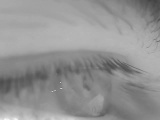
\includegraphics[width=\linewidth]{plots/thresholding/thresholded_eyelid.jpg}
    \caption{Original}
    \end{subfigure} &
    \begin{subfigure}{0.2\linewidth}
    \centering
    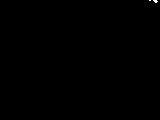
\includegraphics[width=\linewidth]{plots/thresholding/th1}
    \caption{Th = 65}
    \end{subfigure} &
    \begin{subfigure}{0.2\linewidth}
    \centering
    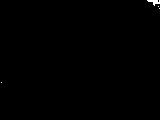
\includegraphics[width=\linewidth]{plots/thresholding/th2}
    \caption{Th = 71}
    \end{subfigure} &
    \begin{subfigure}{0.2\linewidth}
    \centering
    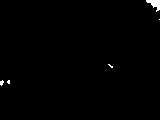
\includegraphics[width=\linewidth]{plots/thresholding/th3}
    \caption{Th = 77}
    \end{subfigure} \\
    \begin{subfigure}{0.2\linewidth}
    \centering
    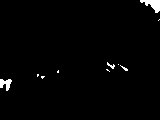
\includegraphics[width=\linewidth]{plots/thresholding/th4}
    \caption{Th = 83}
    \end{subfigure} &
    \begin{subfigure}{0.2\linewidth}
    \centering
    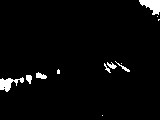
\includegraphics[width=\linewidth]{plots/thresholding/th5}
    \caption{Th = 89}
    \end{subfigure} &
    \begin{subfigure}{0.2\linewidth}
    \centering
    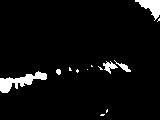
\includegraphics[width=\linewidth]{plots/thresholding/th6}
    \caption{Th = 95}
    \end{subfigure} &
    \begin{subfigure}{0.2\linewidth}
    \centering
    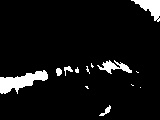
\includegraphics[width=\linewidth]{plots/thresholding/th7}
    \caption{Th = 101}
    \end{subfigure} \\
    \begin{subfigure}{0.2\linewidth}
    \centering
    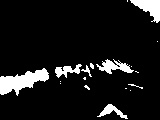
\includegraphics[width=\linewidth]{plots/thresholding/th8}
    \caption{Th = 107}
    \end{subfigure} &
    \begin{subfigure}{0.2\linewidth}
    \centering
    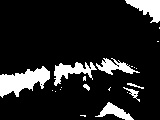
\includegraphics[width=\linewidth]{plots/thresholding/th9}
    \caption{Th = 113}
    \end{subfigure} &
    \begin{subfigure}{0.2\linewidth}
    \centering
    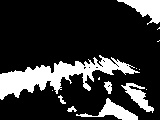
\includegraphics[width=\linewidth]{plots/thresholding/th10}
    \caption{Th = 119}
    \end{subfigure} &
    \begin{subfigure}{0.2\linewidth}
    \centering
    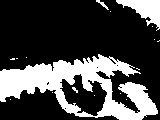
\includegraphics[width=\linewidth]{plots/thresholding/th11}
    \caption{Th = 125}
    \end{subfigure} \\
    \begin{subfigure}{0.2\linewidth}
    \centering
    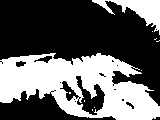
\includegraphics[width=\linewidth]{plots/thresholding/th12}
    \caption{Th = 131}
    \end{subfigure} &
    \begin{subfigure}{0.2\linewidth}
    \centering
    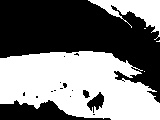
\includegraphics[width=\linewidth]{plots/thresholding/th13}
    \caption{Th = 137}
    \end{subfigure} &
    \begin{subfigure}{0.2\linewidth}
    \centering
    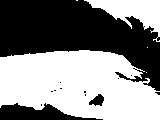
\includegraphics[width=\linewidth]{plots/thresholding/th14}
    \caption{Th = 143}
    \end{subfigure} &
    \begin{subfigure}{0.2\linewidth}
    \centering
    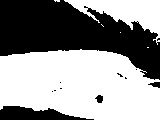
\includegraphics[width=\linewidth]{plots/thresholding/th15}
    \caption{Th = 149}
    \end{subfigure} \\
    \end{tabular}
    \caption{Thresholded images}
    \label{fig:thresholded_images}
    \end{figure}

    \subsubsection{Ellipse fitting}
    \label{subsubsec:ellipsefitting}
    Ellipse fitting \cite{fitzgibbon_direct_2000} based on minimizing the algebraic distance by using least squares fitting is a very common method to fit an ellipse to a set of points. Given a set of $n$ 2D points $p_i = (x_i, y_i)$ where $i = 1,2,...,n$ and the equation of an ellipse in standard form is: 
    \begin{equation}
        F(x,y)=Ax2+Bxy+Cy2+Dx+Ey+F=0
        \label{eq:ellipse_standard}
    \end{equation}
    Where $a=[A, B, C, D, E, F]^T$ are the parameters to be determined. To exclude the trivial solution $a=0$ the constraint $||a||^2=1$ is added. Another important constrain is that the ellipse is actually an ellipse and not a hyperbola or parabola. This is done by adding the constraint $B^2-4AC<0$.
    Let's define the design Matrix $D$ as: 
    \begin{equation}
        D = \begin{pmatrix}
        x_1^2 & x_1y_1 & y_1^2 & x_1 & y_1 & 1 \\
        x_2^2 & x_2y_2 & y_2^2 & x_2 & y_2 & 1 \\
        \vdots & \vdots & \vdots & \vdots & \vdots & \vdots \\
        x_n^2 & x_ny_n & y_n^2 & x_n & y_n & 1 
        \end{pmatrix}
        \label{DesignMatrix}
        \end{equation}
    And let's define $C$ as the constrain matrix so that the constraint can be ex pressed as $a^TCa=1$

        \begin{equation}
            C = \begin{pmatrix}
            0 & 0 & 2 & 0 & 0 & 0 \\
            0 & -1 & 0 & 0 & 0 & 0 \\
            2 & 0 & 0 & 0 & 0 & 0 \\
            0 & 0 & 0 & 0 & 0 & 0 \\
            0 & 0 & 0 & 0 & 0 & 0 \\
            0 & 0 & 0 & 0 & 0 & 0 \\
            \end{pmatrix} \label{eq:C}
        \end{equation}
Now the method of Lagrange multipliers \cite{gander_least_1980} gives the conditions for solving the least squate fit with the scatter matrix being $S=D^TD$: 
\begin{gather}
    Sa = \lambda Ca \\
    a^TCa=1
\end{gather}
This return at most six solutions for $a_j$ and $\lambda_j$. The solution with the smallest $\lambda_k$ and the corresponding eigenvector $a_k$ is the best fit for the ellipse based on the least square fit. 

\subsubsection{Contours}
    When working with thresholds the contour is of interests. The contour is defined as the outer boundary of the threshold binary matrix and is the foundation for the ellipse fit method. 
    Here it is not given to extract one single contour and therefore the contours need to be filtered based on which contour represents the pupil the best. 
    Mainly three criteria are used. 
    
    \paragraph{Circularity / Compactness}
    \begin{equation}
        \frac{4\pi\mathsf{A} }{(\oint_{\partial S} dS)^2}
    \end{equation}
    Where $\mathsf{A} $ is the Area of the contour, and it is divided by the integral over the outer boundary of the contour also known as the permitter of the contour.

    \paragraph{Similarity }
    The for the similarity the OpenCV library is used. This methods compares a given shape with another. As base for the comparison a simple ellipse is taken and then compared.

    \paragraph{Area}
    The Area of the contour should be maximal to find the greatest pupil area and filter out smaller area contours. 

   Each algorithm that returns a list of contours needs them to be checked with these four conditions and in the best case scenario only the contour of the pupil survives. This is then the contour on which a ellipse will be fitted. 

\newpage
\subsection{Random Sample Consensus (RANSAC) }
\label{sus:ransac}
The Random Sample Consensus (RANSAC)\cite{derpanis_overview_nodate} algorithm is an iterative method that is used to estimate the parameters for a known problem. For ellipse fitting a contour or a set of possible points inside or on the contour $C$ is the input. The algorithm then randomly selects a subset $S_c$ of 5 random selected points in $C$. 
These 5 points are then used to fit an ellipse as described in the section Ellipse Fitting.

\begin{figure}[h]
    \centering
    \begin{tikzpicture}[scale=0.4]
        % Drawing the coordinate system
        \draw[->] (-1,0) -- (12,0) node[right] {$x$}; % x-axis
        \draw[->] (0,-1) -- (0,12) node[above] {$y$}; % y-axis
        
        % Drawing the ellipse
        \draw[rotate around={30:(8,8)},scale=1] (8,8) ellipse (7cm and 5cm);
        
        % Annotations
        \node at (8,7) {$(h,k)$};
        \draw [rotate around={30:(8,8)},scale=1] (8,8) -- ++(7,0) node[midway,above] {$a$};
        \draw [rotate around={30:(8,8)},scale=1] (8,8) -- ++(0,5) node[midway,right] {$b$};
        \draw[scale=1, red] (8,8) -- ++(4.5,0) node[midway,above] {$\theta$};
        \draw[scale=1, red] (8,8) ++(4,0) arc (0:30:4);
        \filldraw[black] (8,8) circle (2pt);

    \end{tikzpicture}
    \caption{Ellipse with center $(h,k)$, semi-axes $a$ and $b$, and rotation $\theta$}
    \label{fig:sampleellipse}
\end{figure}

\begin{equation}
    \frac{((x-h)\cos(\theta) + (y-k)\sin(\theta))^2}{a^2} + \frac{((x-h)\sin(\theta) - (y-k)\cos(\theta))^2}{b^2} = 1
    \label{ellipsequation}
\end{equation}

The equation \ref{ellipsequation} represents an ellipse with major axis $a$, minor axis $b$ and the center of the ellipse at $(h,k)$. The angle $\theta$ is the rotation of the ellipse in the coordinate system. When comparing it with the general ellipse equation and compare coefficients the covariance matrix can be derived:
\begin{equation}
    \mathbf{A}x^2 + \mathbf{B}xy + \mathbf{C}y^2 = 1
    \label{ellipseco}
\end{equation} 
\begin{align}
    \mathbf{A}&=a^2 * \sin (\theta)^2 + b^2*\cos (\theta)^2 \\
    \mathbf{B}&= 2(a^2-b^2)*\sin (\theta)*\cos (\theta) \\
    \mathbf{C}&= a^2*\cos (\theta)^2 + b^2*\sin (\theta)^2
    \label{coefficients}
\end{align}
The covariance matrix is then defined as:

\begin{equation}
    \mathbf{V} = \begin{bmatrix}
        \mathbf{A} & \mathbf{B} \\
        \mathbf{B} & \mathbf{C} 
    \label{covariance}
    \end{bmatrix}
\end{equation}
The benefit of using the covariance matrix is, that the eigenvalues and eigenvectors have a direct relation to the major and minor axis and the rotation of the ellipse. The eigenvalues represent the major and minor of the axis and the eigenvectors represent the rotation matrix $R$ to rotate the ellipse in the coordinate system. Important to note is, that the eigenvectors need to be ordered to the size of the eigenvalues. The eigenvector calculated with the bigest eigenvalue comes first. This has the benefit that all parameters are known to transform all points into a new coordinate system where the calculated ellipse equation is represented in an unit circle.

\begin{figure}[h]
    \centering
    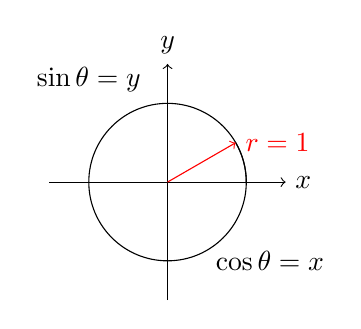
\begin{tikzpicture}
        % Draw the circle with radius 1
        \draw (0,0) circle (1);
        
        % Draw the axes
        \draw[->] (-1.5,0) -- (1.5,0) node[right] {$x$};
        \draw[->] (0,-1.5) -- (0,1.5) node[above] {$y$};
        
        % Define the angle
        \def\angle{30}
        
        % Draw the angle arc
        \draw (1,0) arc (0:\angle:1);
        
        % Draw the line and label
        \draw[->,red] (0,0) -- (\angle:1) node[right] {$r=1$};
        
        % Draw the labels for the trigonometric identities
        \node at (1.3,-1) {$\cos \theta = x$};
        \node at (-1,1.3) {$\sin \theta = y$};

    \end{tikzpicture}
    \caption{Unit circle with trigonometric identities}
    \label{fig:unit_circle}
\end{figure}

This allows for a simple distance calculation. Because $\lambda_{1,2}$ are known, the new coordsystem can be transformed to the unit circle by dividing the x and y values by the eigenvalues. The points form $C$ are then multiplied by the transposed eigenvectors to rotate the points into the new system and then divide by the eigenvalues. Let $p$ be a point in $C$ and $p'$ the transformed point in the new coordinate system. 
\begin{align}
    p' = R^T \begin{bmatrix} p_x - h \\ p_y - k \end{bmatrix} \odot \begin{bmatrix} \frac{1}{\lambda_1} \\ \frac{1}{\lambda_2} \end{bmatrix}\\
    r = \sqrt{p_x'^2 + p_y'^2}
    \label{distance calculation}
\end{align}
So the distance calculation of a point $p$ to the ellipse curve simplifies to the distance of the transformed point $p'$ to the unit circle.
\begin{equation}
    d = \sqrt{p_x'^2 + p_y'^2} -1
\end{equation}

By using this knowledge, the RANSAC algorithm iterates $n$ times to find the best ellipse with the most inliers. The inliers are calculated like following: 
\begin{equation}
    p =\begin{cases}
    \text{inlier} = \{p \in C | d < 0\}\\
    \text{border} = \{p \in C | d = 0\}\\
    \text{outlier} = \{p \in C | d > 0\}
    \end{cases}
    \label{inliers}
\end{equation}
The RANSAC algorithm calculates the ellipse parameters with five random points $S_c$ for $n$ iterations and evaluates each iteration the number of inliers. The ellipse with the most inliers is then used to calculate the final ellipse parameters with the best fit. 
The differentiation between on border an inlier is important to weight the focus on enclosing ellipses or on the border of the ellipse. Because the calculation of the distance $d$ is not an integer, it is possible that the distance is not exactly zero but still on the border. So it is important to keep in mind that comparing floats with each other, to alway use a small epsilon value that d can differ from 0 to set the threshold. 
In python functions like \textit{isclose} from the math module can be used to compare floats with each other. The number of iterations to find a 99\% chance of finding the best ellipse with the most inliers can be calculated with the following formula: 
\begin{equation}
    n = \frac{\log(1-p)}{\log(1-w^s)}
    \label{iterations}
\end{equation}
Where p = is the probability of finding the best ellipse and w is the ratio of inliers to outliers (Probability that a point is an inlier). This formula can then be used to estimate the number of iterations $n$ for the RANSAC algorithm to be 99\% sure to find the best ellipse with size $s$ as sample. In our case we use $s=5$, $p=0.99$ and for $w$ an approximation needs to be made. Because the number of inliers is unknown the ratio of inliers to outliers can not be calculated and needs to be estimated. In this case we assume that the ratio of inliers to outliers is $w=0.90$ which can be adapted later on. 
\begin{equation}
    n = \frac{\log(1-0.99)}{\log(1-0.90^5)} =  5.158
\end{equation}
So the number of iterations to find the best ellipse with the most inliers is 6. But it is important to keep in mind that this is only true if inliers are the sum of border and inliers. Otherwise the number of iterations needs to increase because the ratio inliers to outliers changes drastically. Also an important fact is, that the number of iterations needs to be chosen high enough because throughout the video the number of border points changes drastically and $n$ can not be estimated perfectly. Therefore $n$ is set to $300$ but can still be optimized. If only the border point are considered inliers and only $\frac{1}{5}$ of the border is visible, the number of iterations would jump to $4713$. But not only border points are considered. The calculation of the inliers is discussed in detail in section: \ref{sus:acwe_ransac}
\begin{figure}[h]
    \centering
    \begin{subfigure}{0.3\textwidth}
        \centering
        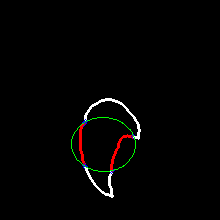
\includegraphics[width=0.9\linewidth]{plots/ransac/test_mask98.png}

    \end{subfigure}%
    \hfill
    \begin{subfigure}{0.3\textwidth}
        \centering
        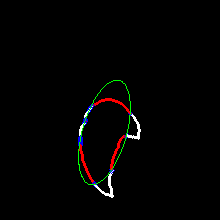
\includegraphics[width=0.9\linewidth]{plots/ransac/test_mask186.png}

    \end{subfigure}%
    \hfill
    \begin{subfigure}{0.3\textwidth}
        \centering
        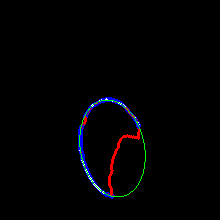
\includegraphics[width=0.9\linewidth]{plots/ransac/test_mask112.png}

    \end{subfigure}%
    \caption{Example of RANSAC ellipse fit iterations}
    \label{fig:RANSAC_it}
\end{figure}

In figure \ref{fig:RANSAC_it} the green ellipse is the ellipse fitted to the five random chosen points. The red points are the inliers of the ellipse and the blue points are the points that lay on the boundary within a given threshold. The white point are the outliers of the ellipse. The number of inliers are the sum of the red points and the number of boundary points are the sum of blue points. The goal is to find the ellipse with the most inliers, boundary points and smalles area. This leads to an enclosing ellipse with minimal area. All points together are the contour of the binary mask recieved from the ACWE algorithm explained in section \ref{sus:acwe}.
\newpage
\subsection{Active Contouring }
Active contour \cite{vondracek_image_2018} segmentation is a method that is used to find the boundary curve of an object given that the object exists. There a many different approaches in active contouring but in this thesis two variants will be discussed. The first one being the classic snakes approach (Kass et al., 1988) \cite{kass_snakes_1988} with a simple energy function and the other variant being the active contouring without edges (ACWE)  based on level sets. In both cases a initial contour is set and through iterative changes tries to find the boundary curve of an object. Each iteration the contour is changed by a small amount and then evaluated with an energy function. The energy function is a measurement of how well the contour is fitting to the edge of the object and in both cases the energy function is minimized.

Let $C(q): [0, 1] \rightarrow \mathbb{R}^2$ be a parametrized planar curve and let $I : [0, a] \times [0, b] \rightarrow \mathbb{R}^+$ be a given image used to detect the object boundaries with active contouring. The classical snakes approach (Kass et al., 1988) \cite{kass_snakes_1988} associates the curve $C$ with an energy given in \refeq{acgd}
But the most basic description for the energy minimization can be summarized in $E_{int}$ and $E_{ext}$ 
\begin{equation}
    E = E_{int} + E_{ext}
    \label{energy}
\end{equation}
\begin{equation}
        E(C) = \underbrace{\alpha \int_0^1 |C'(q)|^2 \, dq + \beta \int_0^1 |C''(q)|^2 \, dq}_{\text{E}_{int}} - \underbrace{\lambda \int_0^1 |\nabla I (C(q))| \, dq}_{\text{E}_{\text{ext}}}
\label{acgd}
\end{equation}
The goal is to minimize the energy function and by doing so the contour $C$ will find local minimals and depending on the sign of $lambda$ be attracted to light or dark edges. The first two terms of the energy describe the intern energy of the contour and the last term describes the external energy. In other words, the intern energy describes the curve smoothness and the external energy describes the relation of the curve to the edge at the curves boundary. In the following the three terms will be discussed in more detail.

To use these Equations, they have to be applied on a discrete grid. The curve $C$ is discretized into $N$ points  $c_i(x_i,y_i)$ with $i \in [0, N-1]$. The energy function is then calculated for each point $C_i$ and summed up to get the total energy of the curve. The energy function is then minimized by changing the position of the points $c_i(x_i,y_i)$ and the process is repeated until the energy function converges. The energy function is minimized by using the gradient descent method. The gradient of the energy function is calculated and the points $c_i(x_i,y_i)$ are changed by a small amount in the direction of the gradient. The gradient descent method is repeated until the energy function converge to a local minimal. 

The formula can be discretized by sampling the initial curve position evenly and then the formula can be expressed as following: 

\begin{equation}
    E = \sum_{i=0}^{N-1} \alpha (c_{i+1} - c_i)^2 + \beta (c_{i+2} - 2c_{i+1} + c_i)^2 - \lambda |\nabla I (c_i)|
\end{equation}
Here it is important to note, that the points are circular, when $i$ is equal to $N-1$ the next point is $c_0$. Therefore the indices can also be interpreted as $c_{(i+1 \bmod N)}$ and $c_{(i+2 \bmod N)}$
\begin{align*}
    \text {substitute:} \begin{cases}
    \sum_{i=0}^{N-1}(c_{i+1} - c_i) = C'(q) \\
    \sum_{i=0}^{N-1}(c_{i+2} - 2c_{i+1} + c_i) = C''(q)
    \end{cases}
\end{align*}

Where $C'(q)$ calculate the length of the curve and $C''(q)$ calculates the curvature of the curve.  

Because the classic snakes implementation searches for the best boundary curve that localy minimizes the energy function, the initial contour need to be initialized close to the best solution. Otherwise the algorithm will converge to a local minimum and not the global minimum. The classic snakes approach searches for the minimal with PDEs that is solved using the steepest descent method which brings performance issues and is prone to terminate early if a local minimum is found. 

\subsubsection{Active Contouring without Edges (ACWE) }
\label{sus:acwe}
In ACWE \cite{vondracek_image_2018} the same principle is used to find the best object boundary. But in this case the energy function is minimized using level sets and morphological operations to solve the PDEs. \ref{muniz} The morphological operation use four different structuring elements. 

\begin{figure}[ht]
    \centering
    \begin{subfigure}[b]{0.23\textwidth}
        \centering
        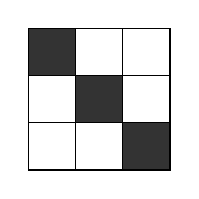
\begin{tikzpicture}[scale=0.6]
            \draw (0,0) grid (3,3);
            \filldraw[fill=black!80] (0,3) rectangle (1,2);
            \filldraw[fill=black!80] (2,0) rectangle (3,1);
            \filldraw[fill=black!80] (1,1) rectangle (2,2);
        \end{tikzpicture}
        \caption{Element 1}
        \label{fig:e1}
    \end{subfigure}%
    \begin{subfigure}[b]{0.23\textwidth}
        \centering
        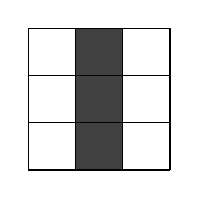
\begin{tikzpicture}[scale=0.6]
            \draw (0,0) grid (3,3);
            \filldraw[fill=black!75] (1,0) rectangle (2,1);
            \filldraw[fill=black!75] (1,2) rectangle (2,3);
            \filldraw[fill=black!75] (1,1) rectangle (2,2);
        \end{tikzpicture}
        \caption{Element 2}
        \label{fig:e2}
    \end{subfigure}
    \begin{subfigure}[b]{0.23\textwidth}
        \centering
        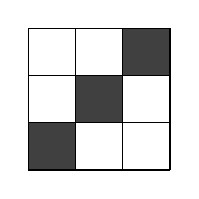
\begin{tikzpicture}[scale=0.6]
            \draw (0,0) grid (3,3);
            \filldraw[fill=black!75] (0,0) rectangle (1,1);
            \filldraw[fill=black!75] (2,2) rectangle (3,3);
            \filldraw[fill=black!75] (1,1) rectangle (2,2);
        \end{tikzpicture}
        \caption{Element 3}
        \label{fig:e3}
    \end{subfigure}%
    \begin{subfigure}[b]{0.23\textwidth}
        \centering
        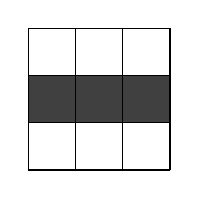
\begin{tikzpicture}[scale=0.6]
            \draw (0,0) grid (3,3);
            \filldraw[fill=black!75] (0,1) rectangle (1,2);
            \filldraw[fill=black!75] (2,1) rectangle (3,2);
            \filldraw[fill=black!75] (1,1) rectangle (2,2);
        \end{tikzpicture}
        \caption{Element 4}
        \label{fig:e4}
    \end{subfigure}%

    \caption{The four morphological structuring elements used in ACWE.}
    \label{fig:neighborsmorph}
\end{figure}
ACWE is based on Geodesic Active Contours (GAC). GAC has the benefit that it already solves key problems from the classical active contouring. Based on thresholds the contour is evaluated and decided if it flows expands the contour to a new pixel or not. GAC is based on classic active contours and geodesic curves in a Riemannian space. The level sets have the benefit that they can easily be implemented in a discrete grid and open the door to solve the PDEs using morphological operations. The level set approach brings more stability and is less sensitive to the initial contour compared to the classical active contouring method. It is also possible to detect the interior and exterior boundary. In the classical approach the interior force is based on first and second derivatives of the curve. This leads to stability, computational complexity and performance issues. This is solved in the GAC by using the evolution of an implicitly defined curve. The GAC algorithm based on a level set function $u$ is defined as following:
\begin{equation}
    \frac{\partial u}{\partial t} = 
    \underbrace{g(I) \cdot |\nabla u| \cdot \text{div} \left(\frac{\nabla u}{|\nabla u|}\right)}_{\text{Smoothing force}} 
    + \underbrace{g(I) \cdot \nu \cdot |\nabla u|}_{\text{Balloon force}} 
    + \underbrace{\nabla g(I) \cdot \nabla u}_{\text{External force}}.
    \label{deform}
    \end{equation}
    
Where $u$ is the level set function, a binary mask that is 1 inside the object and 0 outside. $I$ is the image, $g(I)$ is the edge indicator function, $\nu$ is a variable that decides in which direction and how strong the curve should move. 
For chosing $g(I)$ there are different variants but two of the most common are the following: 

\begin{align}
    g(I) = \begin{cases}
     \frac{1}{1 + |\nabla I|*\alpha} &(1)\\
     \\
     -|\nabla I| &(2)
    \end{cases}
\end{align}
In (1) $g(1)$ is low when the gradient is high and vice versa. Meaning that $g(I)$ regulates the influence of the forces depending on the gradient. It is around 0 when the gradient is high, in other words it stops the curve from moving when the the pixel has reached an edge. $\alpha$ is a variable that regulates how strong the influence of the external energy is.  In (2) $g(I)$ is negative when the gradient is high. So both definition of $g(I)$ will stop the curve from moving when it reaches an edge.

\paragraph{Smoothing force}
The smoothing force is the same as the curvature term in the classical snakes method. The difference is that in GAC the smoothing force is calculated using the gradient of the level set function $u$ instead of the curve. 
\begin{equation}
    g(I) \cdot |\nabla u| \cdot \text{div} \left(\frac{\nabla u}{|\nabla u|}\right)
\end{equation}
Now the smoothing force is calculated with using an recursive call of SI and IS of operator F that approximates the curvature flow that is based on PDE. 
\begin{equation}
    \text{F}(u) = SI(u)\circ IS (u)
    \label{eq:smoothingforce}
\end{equation}
Where SI means supremum of infimum and IS means infimum of supremum. In other words, SI stands for erode and IS stands for dilate. One step of smoothing looks like following: 
\begin{align*}
    1) u_{SI\circ IS}=\text{erode}(u) \circ \text{dilate}(u) \\
    2) u_{IS\circ SI}=\text{dilate}(u) \circ \text{erode}(u)
\end{align*}
by repeating step 1 to 2 the smoothing force can be stronger or weaker. But it is important so always use step 1 and step 2 in the same order. 


\paragraph{Balloon force}
The balloon force is important in regions where the gradient is low and hinders the curve flow to get stuck at a local minimum. Expecially when looking at the external force, where the velocity of the curve is determined by the gradient of $g(I)$ and the gradient of $u$. Ifh $g(I)$ goes to zero the curve will have no external velocity, therefore the balloon force is important to make the algorithm more robust.
\begin{equation}
    g(I) \cdot \nu \cdot |\nabla u|
\end{equation}
To make GAC more computational efficient the ballon force and also the smoothing force are computed differently. 
The Balloon force is $g(I)*|\nabla u| *v$ with parameter $v \in  {-1,1}$ can be substituted with dilation over the four different neighborhood structuring elements. Because dilation is a morphological operation it is computed very efficient and also gets rid of the PDEs that need to be solved in the classical snakes method. By using dialate the balloon force leads to the wanted result by making the curve grow. 
\begin{equation}
    \text{dialate}(u)  =  u \bigoplus Element_i \quad \text{for} \quad i \in \{1,2,3,4\}
    \label{dialate}
\end{equation}

\paragraph{External force}
The external force is the same as in the classical snakes method but in GAC it is weighted by $g(I)$ to stop the curve from moving when it reaches an edge.
\begin{equation}
    \nabla g(I) \cdot \nabla u
\end{equation}
The change in the level set function $u$ is only applied to the points where $g(I) > T$ where $T$ is a defined threshold to control the velocity and the characteristic that the curve moves faster in areas where the gradient is low. This leads to an algorithm that moves faster in a region with the same intensity and slower in regions with a high gradient. 

The external force or the attracting force is calculated for each point $p$ in the binary mask from the before modified level set function $u$ and evaluated with the following equation:
\begin{equation}
    p = \begin{cases}
        1 &iff  \nabla u * \nabla g(I) > 0 \\
        0 &iff \nabla u * \nabla g(I) < 0
    \end{cases}
    \label{eq:externalforce}
\end{equation}
\paragraph{Summary}
To conclude, the equation \refeq{eq:externalforce} describes the deformation of $u$, the binary level set function. and is the main equation for Geodesic Active Contours (GAC). 

\subsubsection{Convert GAC to ACWE}
\label{sus:acwe_ransac}
The GAC only inspects places where the curve could move iteratively and this is the main difference to ACWE. ACWE also known as Chan-Vese algorithm takes the complete image into consideration to evaluate the boundary or the curvature flow of the level set. 
Let $c_i$ the the mean intensity of an subset $Oomega$ of the image $I$ and let $c_1$ be the mean intensity inside the curve or level set $u$ defined as $\Omega_1$ and $c_2$ the mean intensity outside level set $u$ defined as $\Omega_2$. 
\begin{equation}
    c_{i}= \frac{ \int_{\Omega_{i}} I(x) \,dx}{\int_{\Omega_{i}} \, dx }
    \label{eq:meanintensity}
\end{equation}
Then the external force function $F(c_1,c_2,C)$ is defined as
\begin{equation}
    \begin{split}
    F(c_1, c_2, C) = & \mu \cdot \text{length}(u) + \nu \cdot |\text{inside}(u)| \\
    & + \lambda_1 \cdot \int_{\Omega_1} (I(x) - c_1)^2 \, dx \\
    & + \lambda_2 \cdot \int_{\Omega_2} (I(x) - c_2)^2 \, dx
    \end{split}
    \label{eq:curvatureflow}
    \end{equation}

where the first two terms $\mu \cdot \text{length}(u) + \nu \cdot |\text{inside}(u)|$ are the same as in the GAC The third and fourth terms sort of calculate the unscaled intensity variance in the different subsets $\Omega_1$ and $\Omega_2$. 

The only difference now between GAC and the ACWE is that the external forceis is calculated differently. In GAC the external force is calculated with $\nabla g(I) \cdot \nabla u$ and based on a threshold decides if a point is inside or outside the curve, as seen in equation \refeq{eq:externalforce}. 

In ACWE the external force is calculated with the mean intensity of the subsets $\Omega_1$ and $\Omega_2$ and the intensity of the image $I(x)$ as seen in equation \refeq{eq:curvatureflow}. Converting the equation onto an discrete grid it can be written as: 
\begin{equation}
   \xi  = \underbrace{\lambda_{1} \cdot | \nabla u_{mask}| \cdot (I(x)-c_{1})^{2}}_{Inside}-\underbrace{\lambda_{2} \cdot|\nabla u_{mask}| \cdot (I(x)-c_{2})^{2}}_{outside}
\end{equation} 
$\xi$ is then used to calculate the new level set function $u$ with the following equation:
\begin{equation}
    u(x,y) = \begin{cases}
        1 \text{ if } \xi<0 \\
        0 \text{ if } \xi>0 \\
        \text{do nothing otherwise}
        \end{cases}
\end{equation}
The Gradient of the mask will only be nonzero at the contour of the mask. 
Now $I(x)$ is subtracted by the mean and each point on the contour will have two values, their inside and outside weighted intensities. By subtracting the mean intensity from the pixel intensities on the boundary of u, multiplying it with $\lambda_i$ and subtracting the outside term from the inside term an relationship between the inside and outside intensities is created and can be tuned with the sensitivity parameters $\lambda_i$ . 

This relationship is then used to calculate the new level set function $u$ and the process is repeated until the level set function converges. In a case where the function reaches the object boundary the inside and outside intensities will be the same and the curve will not move anymore and the equation goes to zero. 
Here is an example of the evolution the the level set u when the ACWE algorithm is used with a given starting point inside the pupil. 
\begin{figure}[h]
    \centering
    \begin{subfigure}{0.3\textwidth}
        \centering
        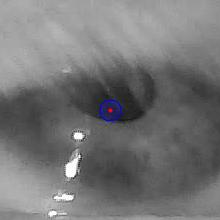
\includegraphics[width=0.9\linewidth]{plots/acwe/iteration_0.png}
        \caption{Initial level set}
    \end{subfigure}%
    \hfill
    \begin{subfigure}{0.3\textwidth}
        \centering
        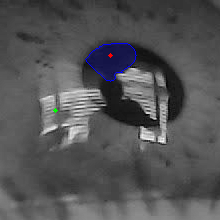
\includegraphics[width=0.9\linewidth]{plots/acwe/iteration_15.png}
        \caption{Iteration 15}
    \end{subfigure}%
    \hfill
    \begin{subfigure}{0.3\textwidth}
        \centering
        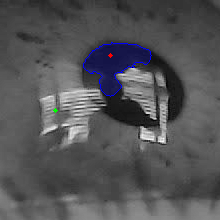
\includegraphics[width=0.9\linewidth]{plots/acwe/iteration_30.png}
        \caption{Iteration 30}
    \end{subfigure}%
    \hfill
    \begin{subfigure}{0.3\textwidth}
        \centering
        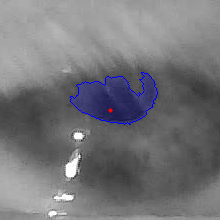
\includegraphics[width=0.9\linewidth]{plots/acwe/iteration_60.png}
        \caption{Iteration 60}
    \end{subfigure}
    \hfill
    \begin{subfigure}{0.3\textwidth}
        \centering
        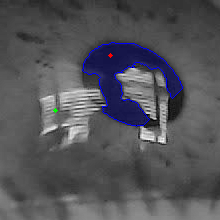
\includegraphics[width=0.9\linewidth]{plots/acwe/iteration_90.png}
        \caption{Iteration 90}
    \end{subfigure}
    \hfill
    \begin{subfigure}{0.3\textwidth}
        \centering
        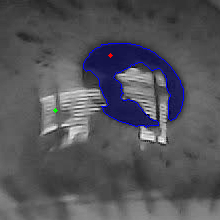
\includegraphics[width=0.9\linewidth]{plots/acwe/iteration_115.png}
        \caption{Iteration 115}
    \end{subfigure}
    \caption{ACWE iterations}
    \label{fig:iterations_acwe}
\end{figure}

\newpage
\subsubsection{Active contouring with ellipse parameters}
A different approach is to let an ellipse grow and modify its parameters based on the gradient information. By sampling an amount of equally spaced points on the ellipse and evaluate an energy function based on the image intensity gradient and the normal vector of the ellipse at those points. The energy function can be described as the scalar product of the gradient and the normal vector of the ellipse curve. 
\begin{equation}
    E = -\sum_{i=0}^{N-1} \nabla I(p_i) \cdot \vec{n(p_i)}
\end{equation} 
Where $p_i$ is a point on the ellipse and $\vec{n(p_i)}$ is the normal vector of the ellipse at that point. $\nabla I(p_i)$ is the gradient of the image at that point. The energy function is minimized by changing the ellipse parameters
\begin{figure}[h]
    \centering
    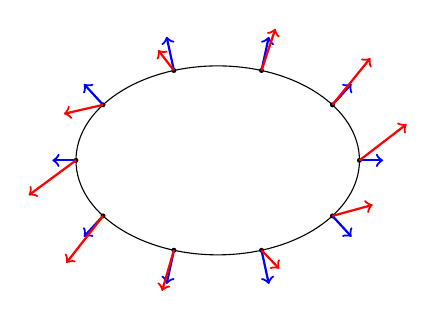
\begin{tikzpicture}[scale=0.6, transform shape]
        \def\a{3} % semi-major axis
        \def\b{2} % semi-minor axis
        \def\scale{1} % scale for normal and gradient vectors
    
        % Draw ellipse
        \draw (0,0) ellipse (\a cm and \b cm );
        
        % Draw 10 points and corresponding vectors
        \foreach \i in {1,2,...,10} {
            \pgfmathsetmacro{\angle}{\i*36}
            \pgfmathsetmacro{\xcoord}{\a*cos(\angle)}
            \pgfmathsetmacro{\ycoord}{\b*sin(\angle)}
            \coordinate (p\i) at (\xcoord,\ycoord);
            \fill (p\i) circle (1.5pt);
    
            % Normal vector
            \draw[->, blue, thick] (p\i) -- ++({\xcoord/\a^2*1.5*\scale},{\ycoord/\b^2*1.5*\scale});
    
            % Dummy gradient vector
            \draw[->, red, thick] (p\i) -- ++({\scale*cos(\angle+\i*0.5)},{\scale*sin(\angle+45+\i*0.5)});
        }
    \end{tikzpicture}
    \label{fig:normalgradientellipse}
    \caption{Ellipse with normal vector (blue) and gradient vectors (red)}
    
    \end{figure}
This converts the problem into a minimization problem. The energy function still needs a term to make sure that the curve grows and does not get stuck at a local minimum. Here it is not possible to use the morphological operators because the shape of the ellipse is not given as a level set. Instead the ellipse is based on only the five ellipse parameter: center$(x,y)$, axis: $(a,b)$ , angle $\theta$. 

The energy function is the lowest when at each point the gradient vector and normal vector  point in the same direction. The gradient vector consists of the magnitude of the gradient and the orientation. Whereas the normal vector is normalized and points in the direction of the normal of the ellipse at that point. 

The problem with this approach is overlapping with the classical active contouring. The initial contour needs to be close to the optimal solution. Otherwise the algorithm stops at an local minimum and convergence to the optimal solution is not guaranteed. Because it is an minimization with five parameters it is a very complex problem and the algorithm needs to be run multiple times to find the best local solution. 

For this approach, the image needs preprocessing and the algorithm is very sensitive to noise. Therefore it is a must to first apply a low pass filter onto the image. But because of blurring the image gradients and directions aren't as accurate as the could be and struggles with reflections and other noise.

Here is an example with the convergence to an local minimum. The initial ellipse is nowhere near to the optimal solution and the algorithm converges to an local minimum. 

\begin{figure}[h]
    \centering
    \begin{tabular}{cc}
        \centering
        \begin{subfigure}{0.3\textwidth}
            \centering
            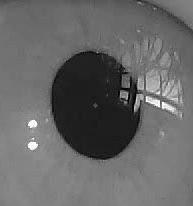
\includegraphics[width=0.9\linewidth]{plots/eye_dataset/roi.png}
            \caption{ROI}
        \end{subfigure} &
        \begin{subfigure}{0.3\textwidth}
            \centering
            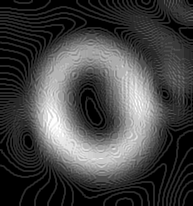
\includegraphics[width=0.9\linewidth]{plots/eye_dataset/mag.png}
            \caption{Gradient Magnitude}
        \end{subfigure} \\
        \begin{subfigure}{0.3\textwidth}
            \centering
            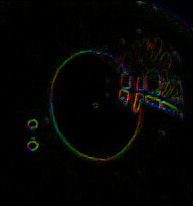
\includegraphics[width=0.9\linewidth]{plots/eye_dataset/direction.png}
            \caption{Gradient Direction}
        \end{subfigure}   &
        \begin{subfigure}{0.3\textwidth}
            \centering
            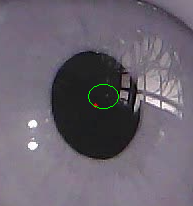
\includegraphics[width=0.9\linewidth]{plots/eye_dataset/result.png}
            \caption{Result}
        \end{subfigure}

    \end{tabular}
    \caption{Convergence to local minimum}
    \label{fig:ac_ellipse_gradient}
    \end{figure}

The problem with expanding the energy function with more terms is, that the algorithm gets more complex. For example when the size is used as a reward for the energy function (the bigger the better), it is not given anymore to stop at the boundary of the object. The parameters have to be chosen smart and carefully to make sure that the algorithm still converges to the optimal solution. 

